% Figure 1 — Framework Diagram (TikZ)
% -----------------------------------------------------------------------------
% Purpose: Publishable workflow diagram for the manuscript:
%          Elicit → TSMM (Stage 1 → Stage 2) → Diagnostics → (optional Dual-Anchor) → Report
%
% Modified: Stage 1 and Stage 2 arranged horizontally within TSMM meta-box
%           to create a more square-shaped figure for manuscript
%
% How to compile:
%   pdflatex -interaction=nonstopmode -halt-on-error Figure_01_framework.tex
%
% Outputs:
%   - Figure_01_framework.pdf (vector)
%
% Author: JoonHo Lee
% Date: 2026-01-15
% -----------------------------------------------------------------------------
\documentclass[tikz,border=3pt]{standalone}

\usepackage{amsmath, amssymb}
\usetikzlibrary{arrows.meta, positioning, shapes.geometric, fit, backgrounds}

\begin{document}
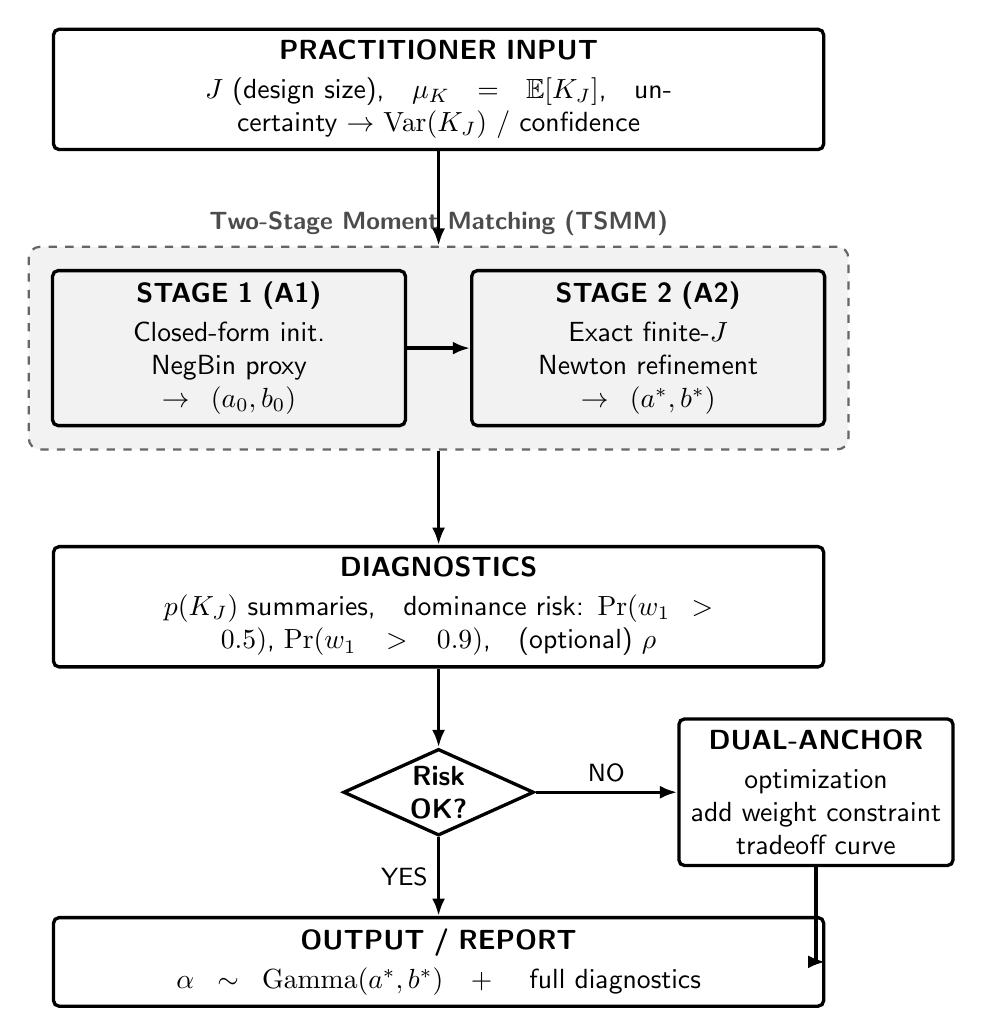
\begin{tikzpicture}[
  font=\sffamily,
  node distance=10mm and 8mm,
  >={Latex[length=2.2mm]},
  % Wide box style (for Input, Diagnostics, Output)
  box/.style={
    rectangle,
    rounded corners=2pt,
    draw=black,
    very thick,
    align=center,
    text width=9.5cm,
    inner sep=4pt
  },
  % Square-ish box style (for Stage 1, Stage 2)
  boxStage/.style={
    rectangle,
    rounded corners=2pt,
    draw=black,
    very thick,
    align=center,
    text width=4.2cm,
    minimum height=1.8cm,
    inner sep=4pt
  },
  % Small box style (for Dual-Anchor)
  boxSmall/.style={
    rectangle,
    rounded corners=2pt,
    draw=black,
    very thick,
    align=center,
    text width=3.2cm,
    inner sep=4pt
  },
  % Meta-box style (for TSMM)
  metabox/.style={
    rectangle,
    rounded corners=4pt,
    draw=black!60,
    thick,
    dashed,
    fill=black!5,
    inner sep=8pt
  },
  % Decision diamond style
  decision/.style={
    diamond,
    draw=black,
    very thick,
    aspect=2.2,
    align=center,
    inner sep=1pt
  },
  lab/.style={font=\sffamily\small}
]

% --- Stage 1 and Stage 2 (side by side) ---
\node[boxStage] (a1) {
  \textbf{STAGE 1 (A1)}\\[2pt]
  Closed-form init.\\
  NegBin proxy\\
  $\rightarrow (a_0, b_0)$
};

\node[boxStage, right=of a1] (a2) {
  \textbf{STAGE 2 (A2)}\\[2pt]
  Exact finite-$J$\\
  Newton refinement\\
  $\rightarrow (a^*, b^*)$
};

% --- TSMM Meta-box (wrapping Stage 1 and Stage 2) ---
\begin{scope}[on background layer]
  \node[metabox, fit=(a1)(a2), 
        label={[font=\sffamily\small\bfseries, text=black!70]above:Two-Stage Moment Matching (TSMM)}] (tsmm) {};
\end{scope}

% --- Practitioner Input (above TSMM) ---
\node[box, above=12mm of tsmm] (input) {
  \textbf{PRACTITIONER INPUT}\\[2pt]
  $J$ (design size),\quad $\mu_K=\mathbb{E}[K_J]$,\quad 
  uncertainty $\rightarrow$ $\mathrm{Var}(K_J)$ / confidence
};

% --- Diagnostics (below TSMM) ---
\node[box, below=12mm of tsmm] (diag) {
  \textbf{DIAGNOSTICS}\\[2pt]
  $p(K_J)$ summaries,\quad 
  dominance risk: $\Pr(w_1>0.5)$,\ $\Pr(w_1>0.9)$,\quad
  (optional)\ $\rho$
};

% --- Decision diamond (below Diagnostics) ---
\node[decision, below=of diag] (dec) {\textbf{Risk}\\\textbf{OK?}};

% --- Dual-Anchor (right of Decision) ---
\node[boxSmall, right=18mm of dec] (dual) {
  \textbf{DUAL-ANCHOR}\\[2pt]
  optimization\\
  add weight constraint\\
  tradeoff curve
};

% --- Output (below Decision) ---
\node[box, below=of dec] (out) {
  \textbf{OUTPUT / REPORT}\\[2pt]
  $\alpha \sim \mathrm{Gamma}(a^*, b^*)$\quad + \quad full diagnostics
};

% --- Arrows ---

% Input → TSMM (single arrow to meta-box)
\draw[->, very thick] (input) -- (tsmm);

% Stage 1 → Stage 2 (inside TSMM)
\draw[->, very thick] (a1) -- (a2);

% TSMM → Diagnostics
\draw[->, very thick] (tsmm) -- (diag);

% Diagnostics → Decision
\draw[->, very thick] (diag) -- (dec);

% Decision → Output (YES branch)
\draw[->, very thick] (dec) -- node[lab, left]{YES} (out);

% Decision → Dual-Anchor (NO branch)
\draw[->, very thick] (dec) -- node[lab, above]{NO} (dual);

% Dual-Anchor → Output
\draw[->, very thick] (dual) |- (out);

\end{tikzpicture}
\end{document}
